% in comparison of diff time lengths
% \subsubsection{Mathmatical Evaluation and Comparison of different time lengths}
% !!! todo: calinski harabasz - as said in document - higher score indicates better clustering (not directly said in paper - but can see in graphs on page 24)

The three mathematical evaluation scores mentioned in section \ref{section:TheoryEvaluatingClusteringResults}, i.e. Silhouette Coefficient, Davies-Bouldin Index, and Caliński-Harabasz Index were used to compare the resulting clusters.  They were each implemented using the sklearn library\footnote{\url{https://scikit-learn.org/stable/modules/generated/sklearn.metrics.silhouette_score.html}, \url{https://scikit-learn.org/stable/modules/generated/sklearn.metrics.davies_bouldin_score.html}, and \url{https://scikit-learn.org/stable/modules/generated/sklearn.metrics.calinski_harabasz_score.html}}, the same way as in section \ref{section:experimentTSNE}.
As also explained in the respective sklearn documentations, the Silhouette Score indicates better, denser clustering, when it is closer to 1, and incorrect clustering results if the value is close to -1. The Davies-Bouldin Index indicates well chosen clusters, when the value is closer to 0 (lowest possible score). A higher Caliński-Harabasz Index suggests well separated and dense clusters.
These three scores were calculated and stored for each data frame, after each clustering algorithm was applied (DBSCAN and OPTICS) for each time length. The resulting values where then compared and are depicted in figures below. 
The experiment was run on each time length (1h files: 15 min, 30 min, 45 min, 1h; 3h files: 30 min, 1h, 1 h 30 min, 2h, 2h 30 min, 3h).
The numbers were different for each time the results were calculated, since t-SNE produces slightly different results. Therefore, the t-SNE and clustering was run multiple times and the results were compared. In appendix \ref{appendix:clusteringEvaluationResults} figures \ref{figure:clusteringResults1} and \ref{figure:clusteringResults2} two individual t-SNE and clusterings were run, figure \ref{figure:clusteringResults3} depicts the average scores of these two. Figure \ref{figure:clusteringResults4} depicts an average of a different two runs. These mentioned runs all held the learning rate parameter 20. Since 800 also proved to be a viable choice for this parameter, the t-SNE and clustering was also run twice and averaged (figure \ref{figure:clusteringResults5}) with a learning rate of 800. The mean was taken from all these revealed results, thus creating figure \ref{figure:clusteringResults6} (the figure can be seen in this section). From these, there is no clear winner, although there are some stronger candidates, i.e. 15 min (1h), 30 min (1h), 1h (3h), and 2h (3h). 

Like before, when comparing the t-SNE results, the light green field indicate the best and most distinct clusters from the 1h or 3h data files, while the dark green fields highlight the best value for that score overall for all time lengths. These green fields, or number of "wins" were summed to see which time length had the best number of scores the most. The light green wins (1h or 3h) for the 1h data files are pictured in figure \ref{figure:clusteringResultsGraph1h}, in figure \ref{figure:clusteringResultsGraph3h} for the 3 hour data files, and in figure \ref{figure:clusteringResultsGraphTotal} for the comparison of the dark green wins (1h and 3h). The two top winners for the 1h data files and the 3h data files, were: 30 min (1h), 15 min (1h), 2h (3h), and 1h (3h). The top four results when comparing all time lengths, despite which files they were aggregated to, were: 30 min (1h), 1h (3h), 2h (3h), and 30 min (3h). The number of "wins" is to some extent reliable on the resulting scores from other time lengths it happened to be compared with. It also does not fully factor in the full scale by how far this time length was better. For this reason, the average scores from figure \ref{figure:clusteringResults6} for thee five "winning" time lengths were compared solely to each other. The results are detailed in figure \ref{figure:clusteringResults8}. The 2h time delta achieved the majority of best scores in this final comparison. When removing the 2h column, 30 min (1h) and 1h (3h) come in second place. 1h (3h) however out performs when compared directly to 30 min (1h).

% 30 1, 15, 2h, 1h (3), 30 min (3)

% 30 min and 2hrs best

% The first block (\textbf{lines...}) shows the results for the 1h data set, the second block (\textbf{lines...}) for the 3h data set, and the last block (\textbf{lines...}) compares the two (for the 1h and 3h time lengths). The light green field indicates, that from the data files (1h or 3h), this time length achieved the best and most distinct clusters, according to that score. Dark green fields highlight the best value for that score overall for all time lengths.

% Counted wins
% Figure \ref{figure:clusteringResults1} 1st run 20
% Figure \ref{figure:clusteringResults2} 2nd run 20
% Figure \ref{figure:clusteringResults3} average 1st and second 20
% Figure \ref{figure:clusteringResults4} 2 average of 20
% Figure \ref{figure:clusteringResults5} 2 average of 800
% Figure \ref{figure:clusteringResults6} averages (1 and 2 run 20, 2 average 20, 2 average 800)
% Figure \ref{figure:clusteringResults7} 1h vs 3h file
% Figure \ref{figure:clusteringResults8} winners comparison
% Figure \ref{figure:clusteringResults9} check - compare all - do need? 



% \begin{figure}
%   \centering
%   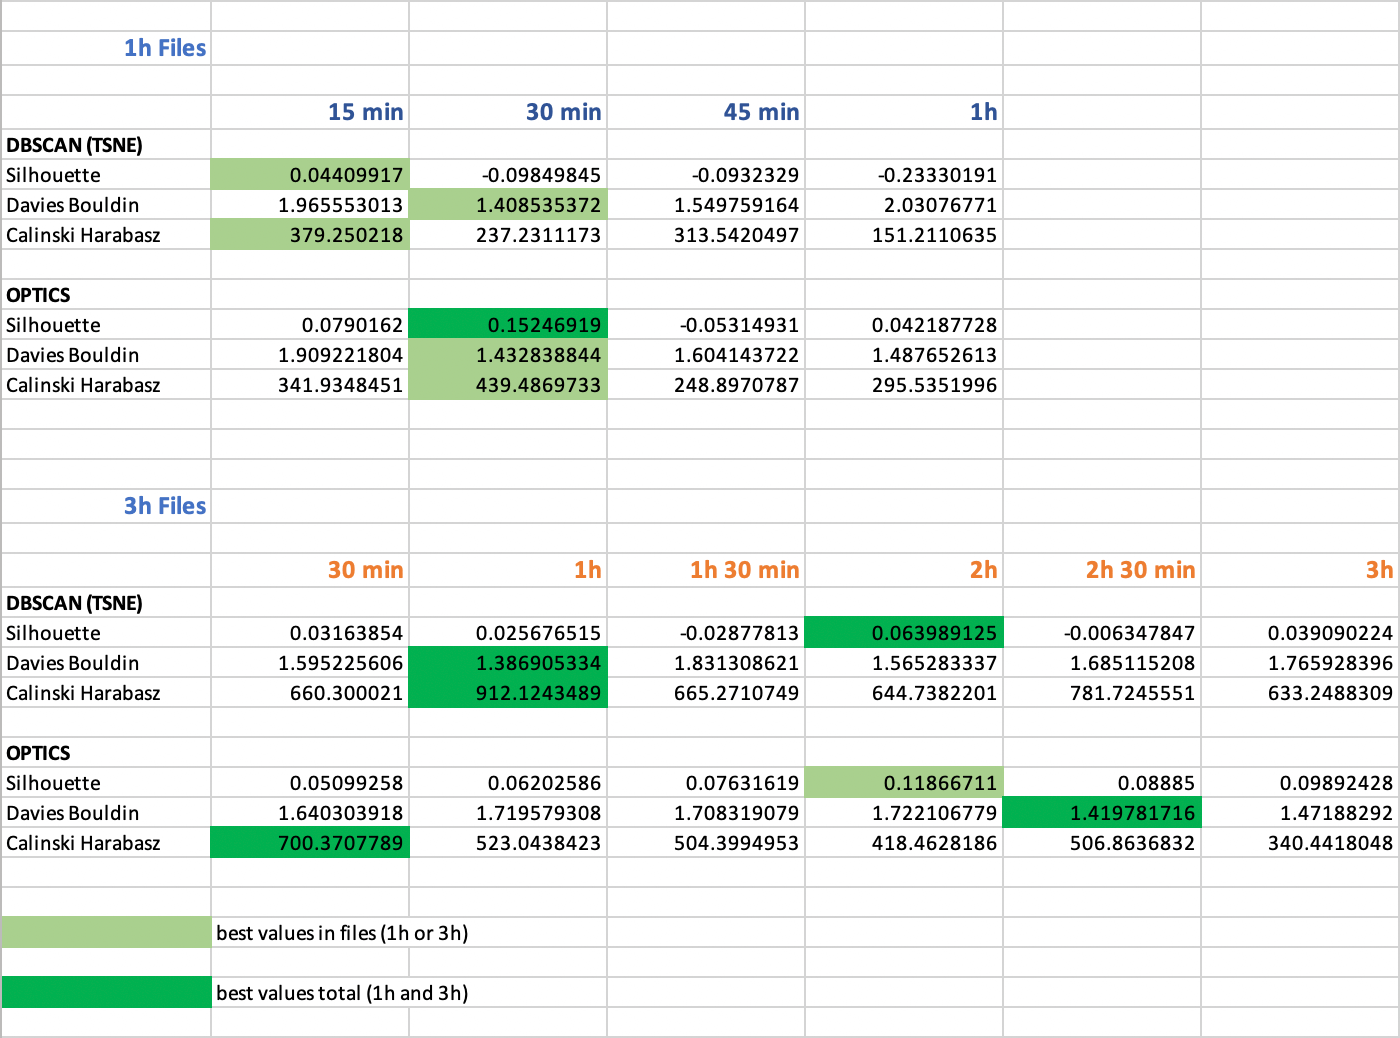
\includegraphics[width=0.8\textwidth]{./images/clusteringResults/clusteringResults1.png}
%   \caption{Evaluation scores comparison from 1h run of t-SNE and clustering with a learning rate of 20.}
%   \label{figure:clusteringResults1}
% \end{figure}

% \begin{figure}
%   \centering
%   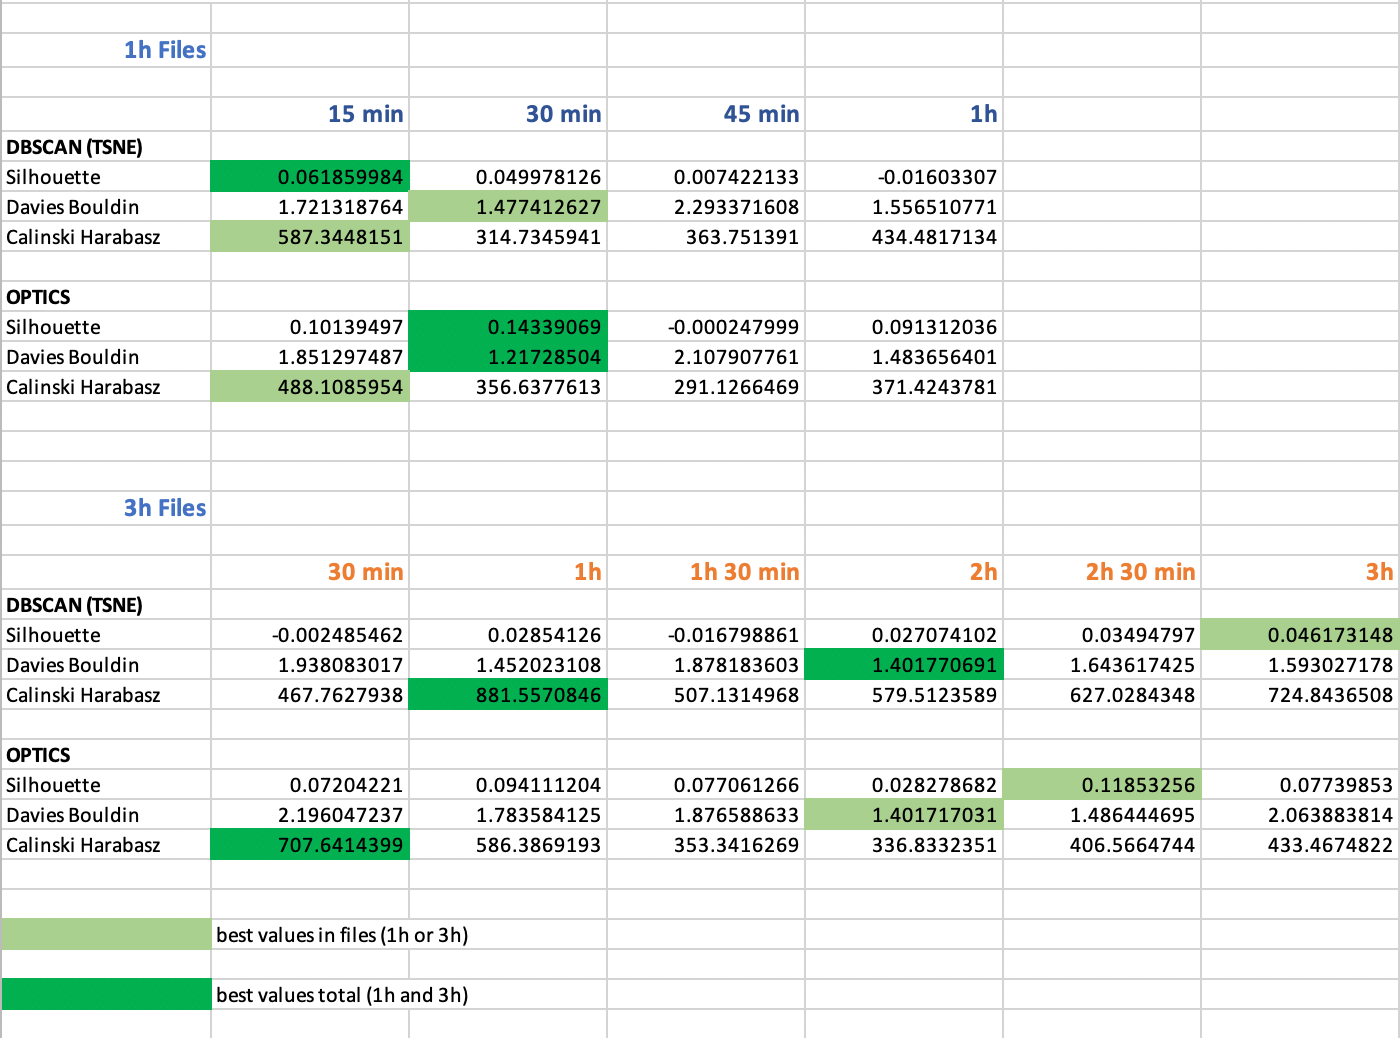
\includegraphics[width=0.8\textwidth]{./images/clusteringResults/clusteringResults2.png}
%   \caption{Evaluation scores comparison from 1h run of t-SNE and clustering with a learning rate of 20.}
%   \label{figure:clusteringResults2}
% \end{figure}


% \begin{figure}
%   \centering
%   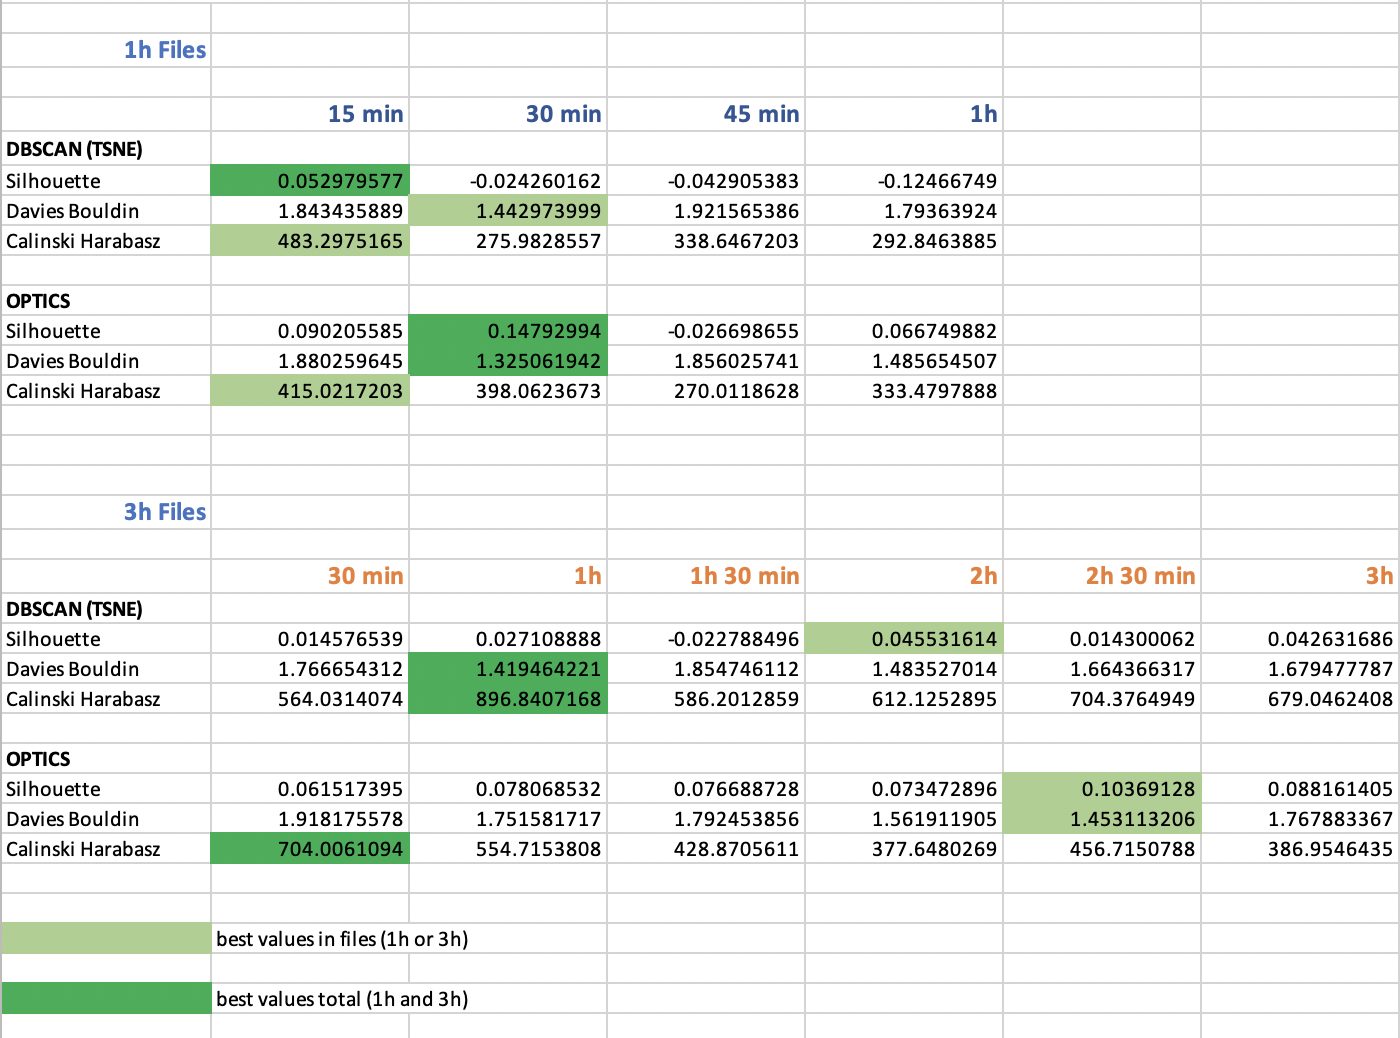
\includegraphics[width=0.8\textwidth]{./images/clusteringResults/clusteringResults3.png}
%   \caption{Evaluation scores comparison averaged from figures \ref{figure:clusteringResults1} and \ref{figure:clusteringResults2}}
%   \label{figure:clusteringResults3}
% \end{figure}

% \begin{figure}
%   \centering
%   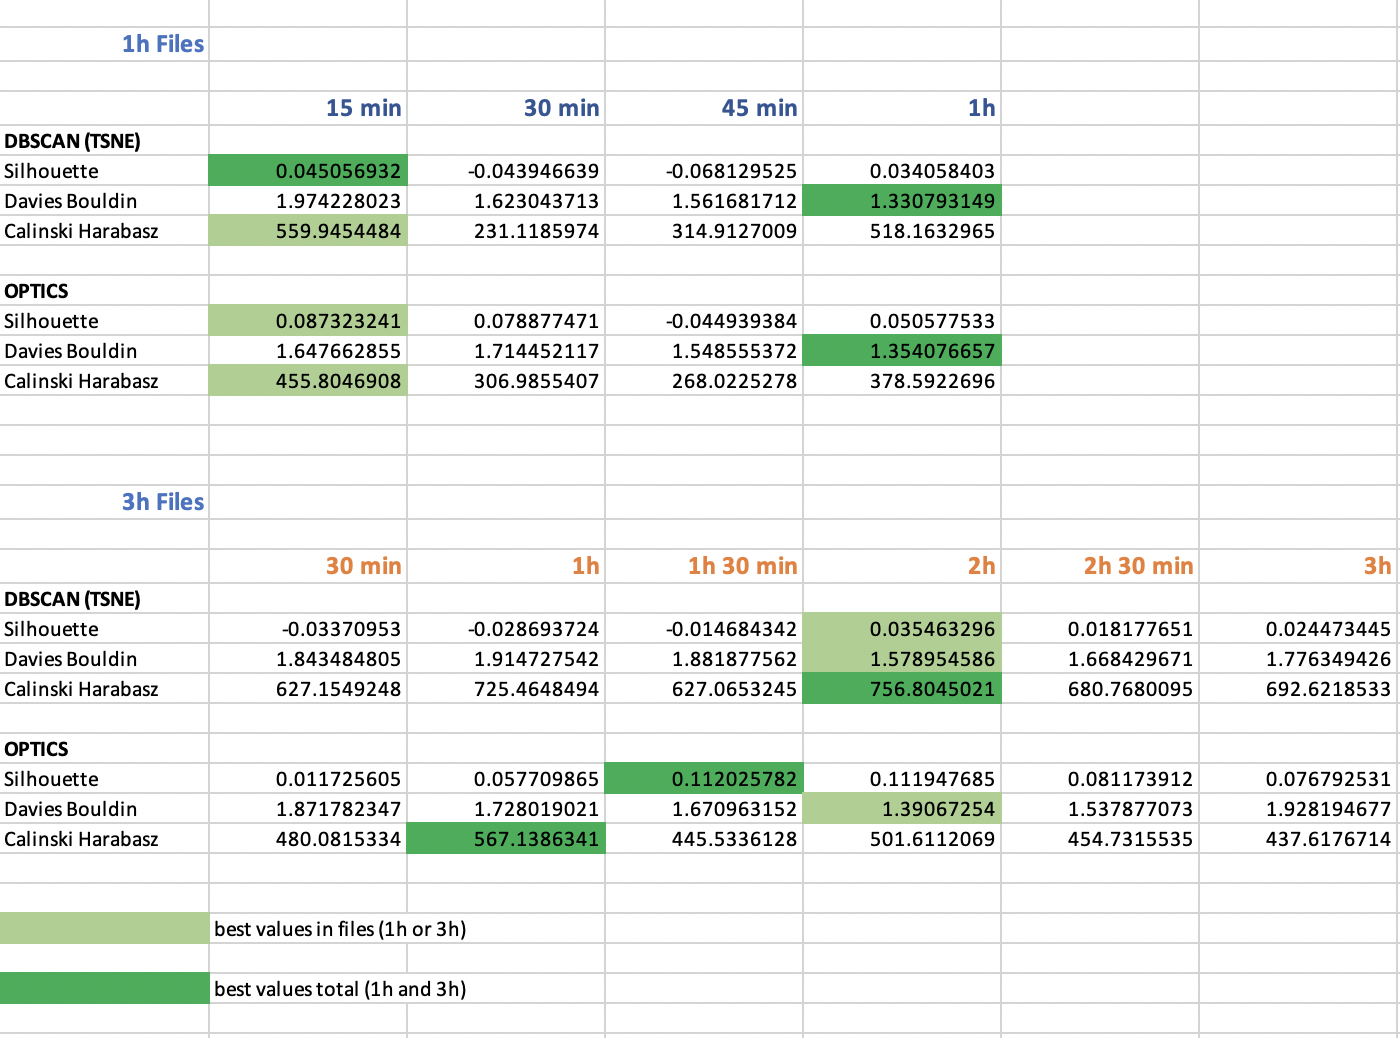
\includegraphics[width=0.8\textwidth]{./images/clusteringResults/clusteringResults4.png}
%   \caption{Evaluation scores comparison averaged from 2 runs of t-SNE and clustering with a learning rate of 20.}
%   \label{figure:clusteringResults4}
% \end{figure}

% \begin{figure}
%   \centering
%   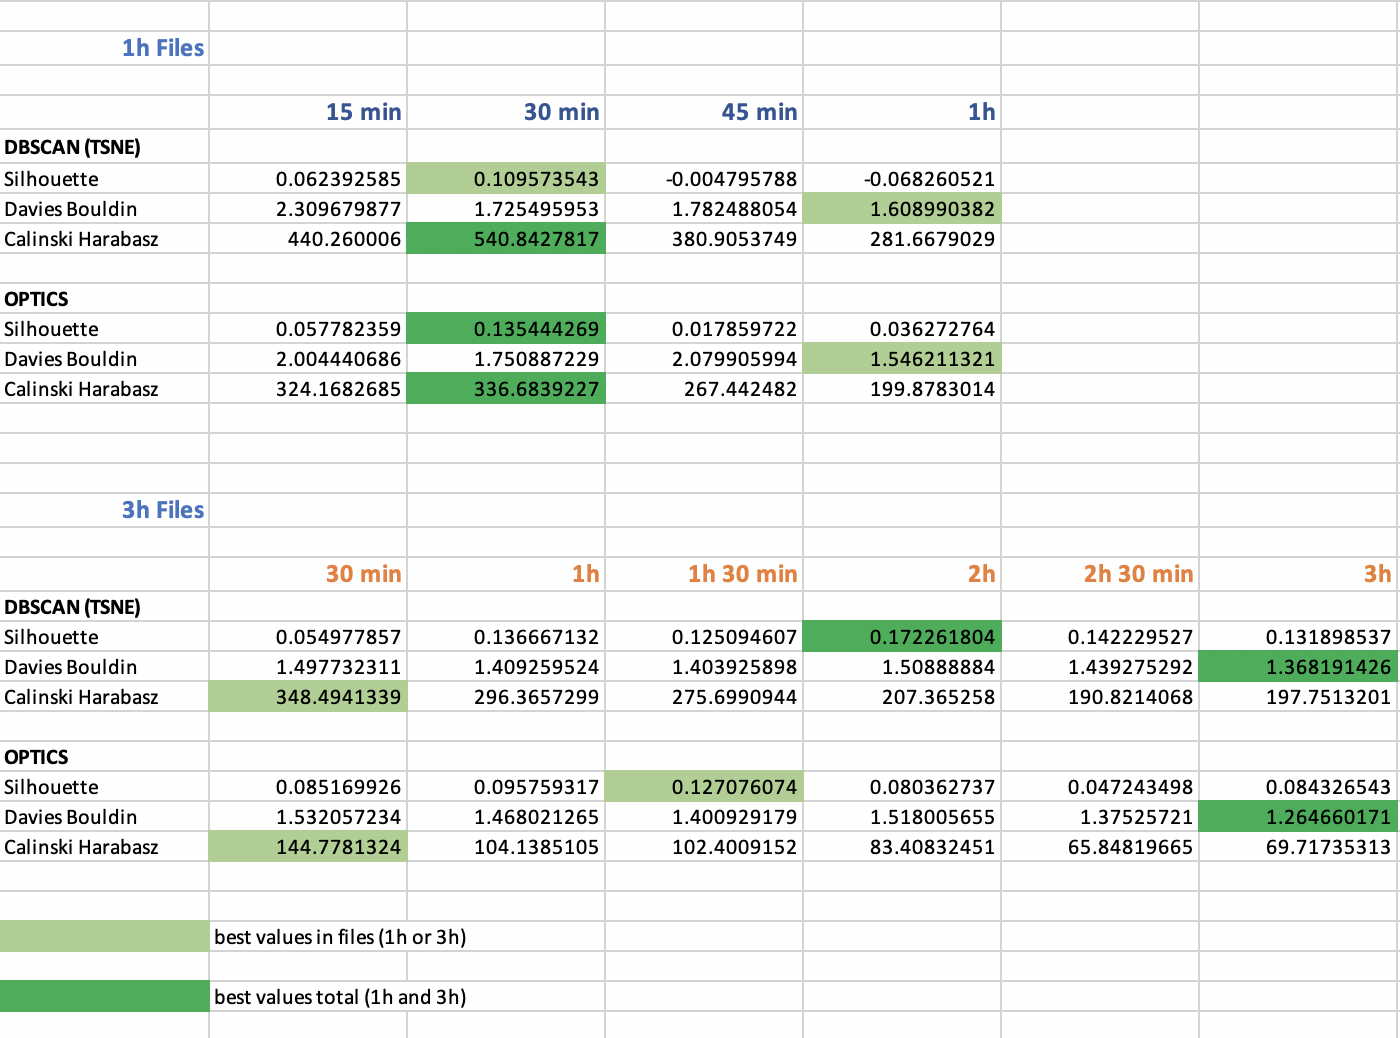
\includegraphics[width=0.8\textwidth]{./images/clusteringResults/clusteringResults5.png}
%   \caption{Evaluation scores comparison averaged from 2 runs of t-SNE and clustering with a learning rate of 800.}
%   \label{figure:clusteringResults5}
% \end{figure}

\begin{figure}
  \centering
  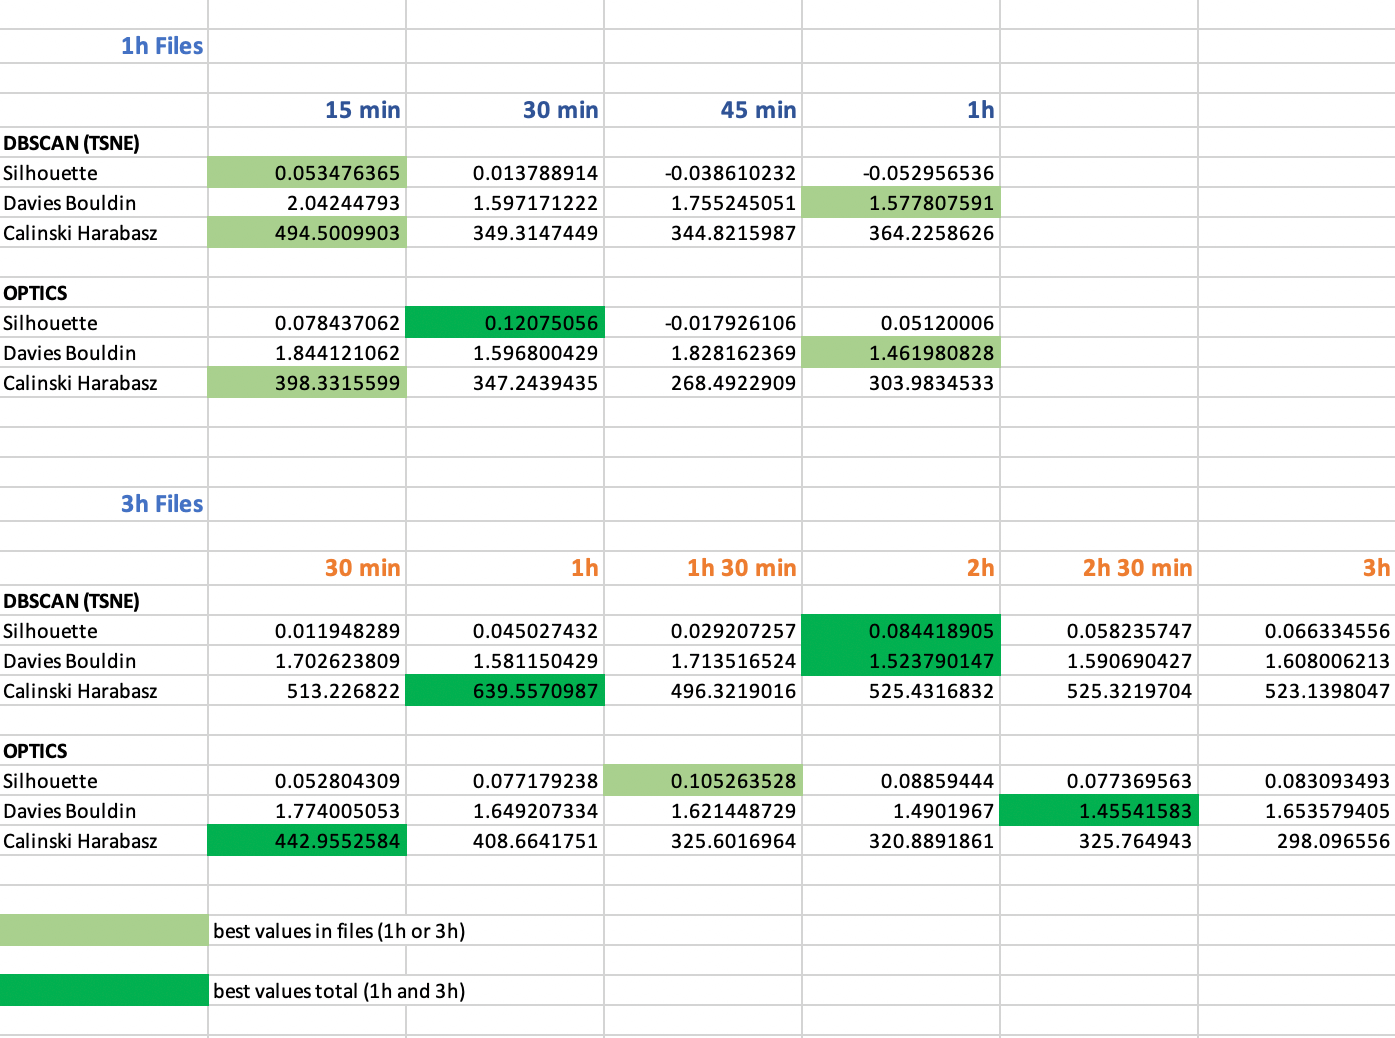
\includegraphics[width=0.8\textwidth]{./images/clusteringResults/clusteringResults6.png}
  \caption{Evaluation scores comparison averaged from figures \ref{figure:clusteringResults1}, \ref{figure:clusteringResults2}, \ref{figure:clusteringResults3}, \ref{figure:clusteringResults4}, and \ref{figure:clusteringResults5}.}
  \label{figure:clusteringResults6}
\end{figure}




\begin{figure}[H]
  \centering
  \begin{subfigure}{.475\textwidth}
    \centering
    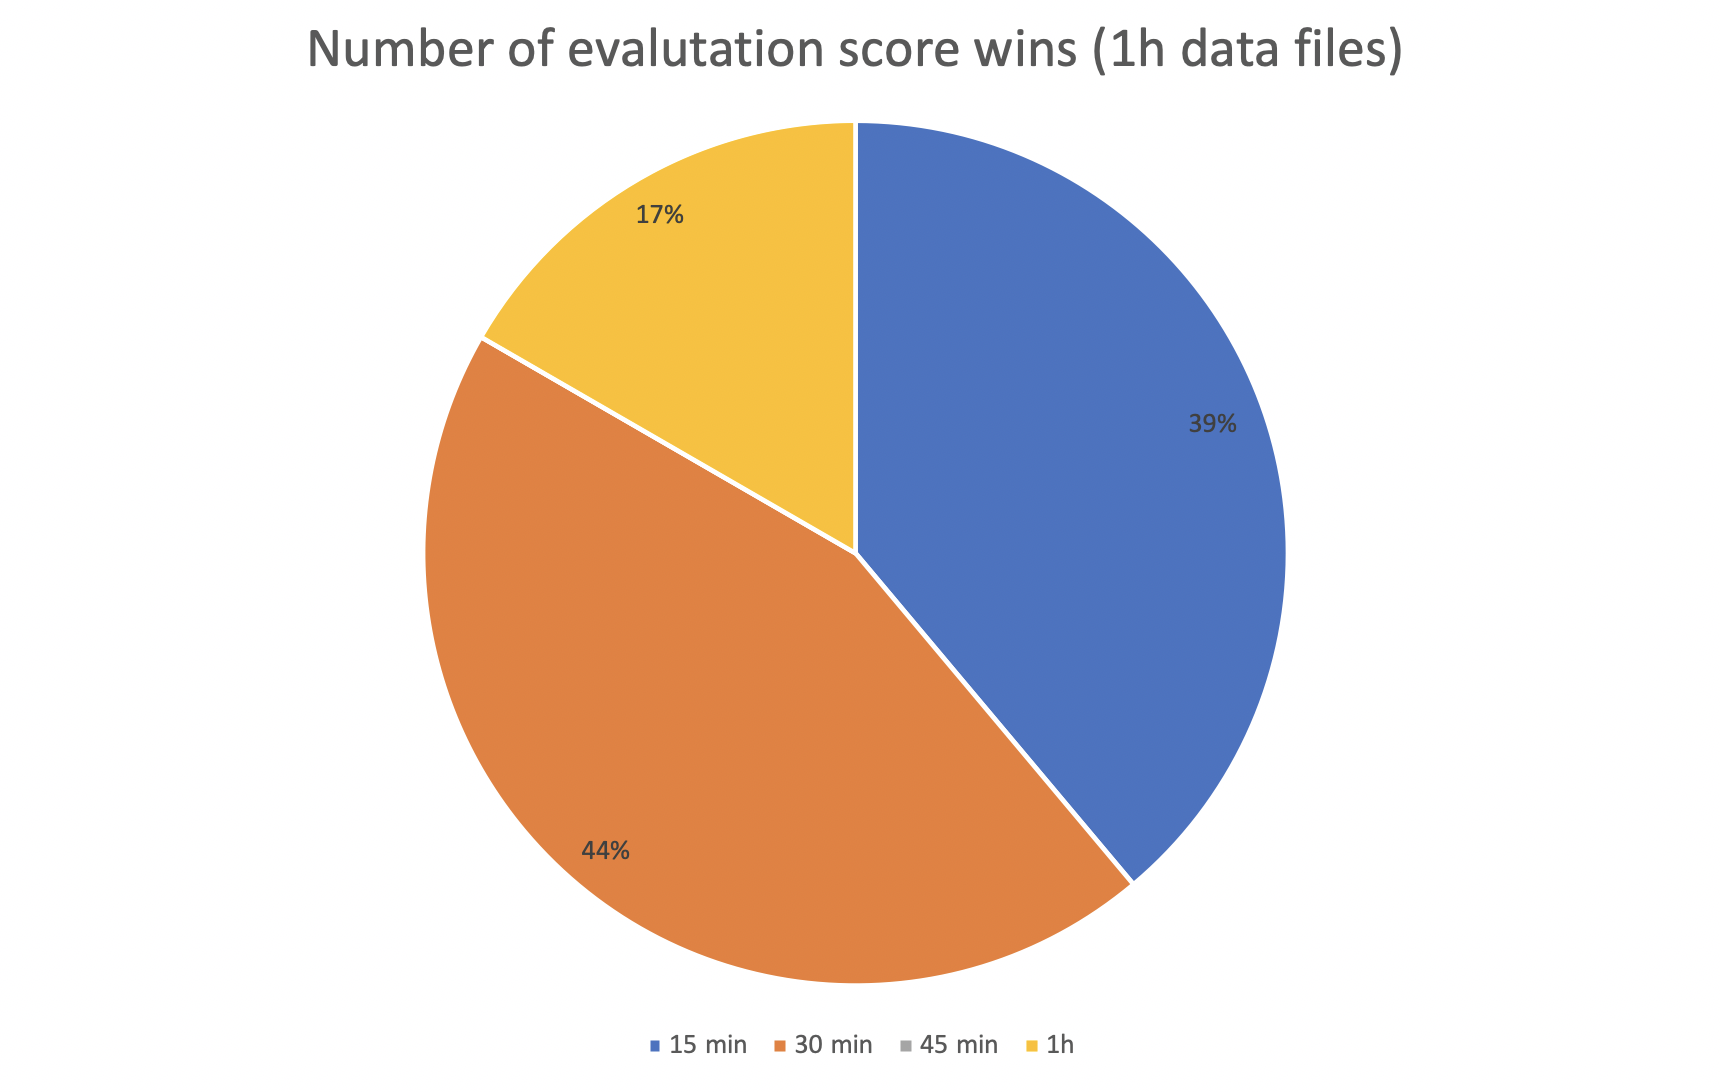
\includegraphics[width=0.8\textwidth]{./images/clusteringResults/clusteringResultsGraph1h.png}
    \caption{Number of light green evaluation score "wins" (1h or 3h) for the 1h data files.}
    \label{figure:clusteringResultsGraph1h}
  \end{subfigure}%
  \hfill
  \begin{subfigure}{.475\textwidth}
    \centering
    \  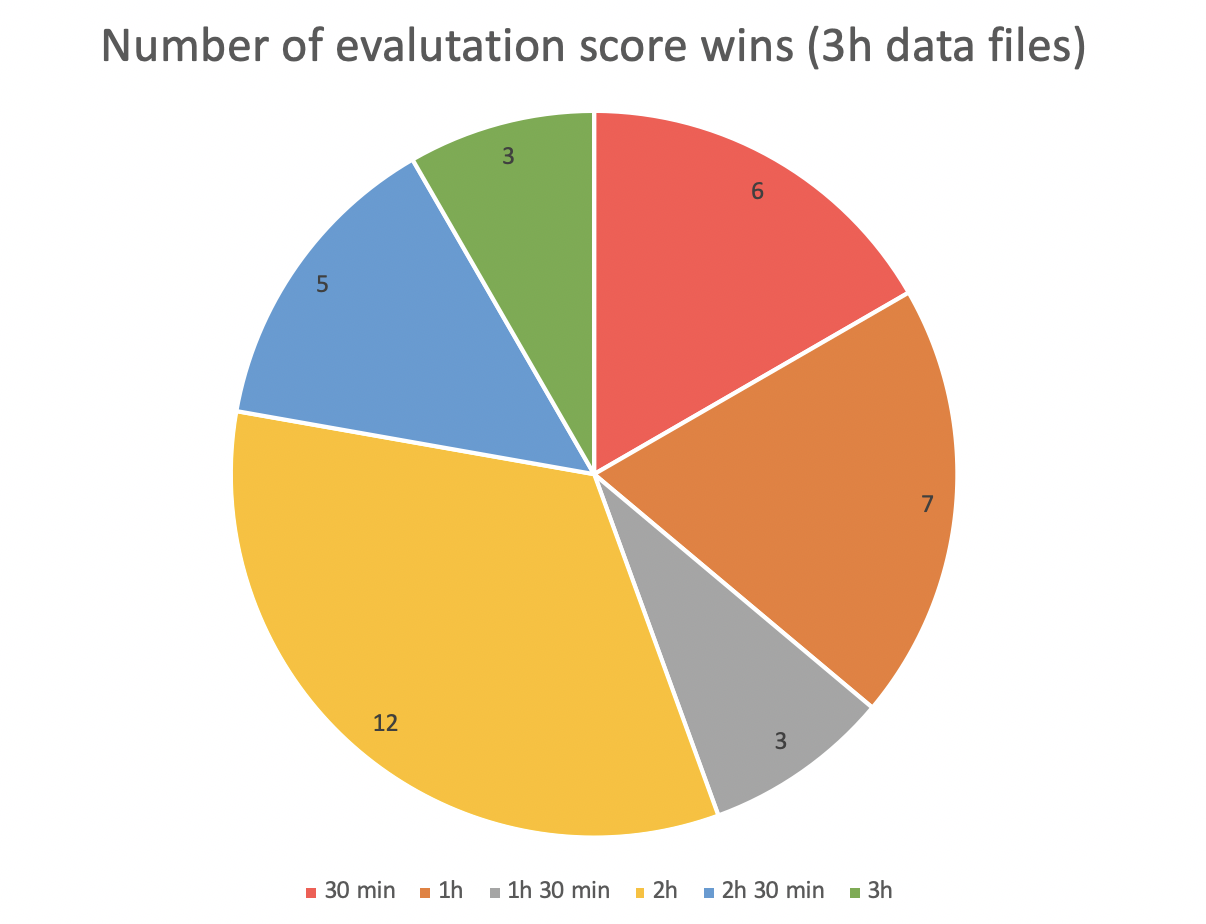
\includegraphics[width=0.8\textwidth]{./images/clusteringResults/clusteringResultsGraph3h.png}
    \caption{Number of light green evaluation score "wins" (1h or 3h) for the 3h data files.}
    \label{figure:clusteringResultsGraph3h}
  \end{subfigure}
	% \caption{Number of light green evaluation score "wins" (1h or 3h) for the 3h data files.}
  % \label{figure:PCA}
\end{figure}


% \begin{figure}
%   \centering
%   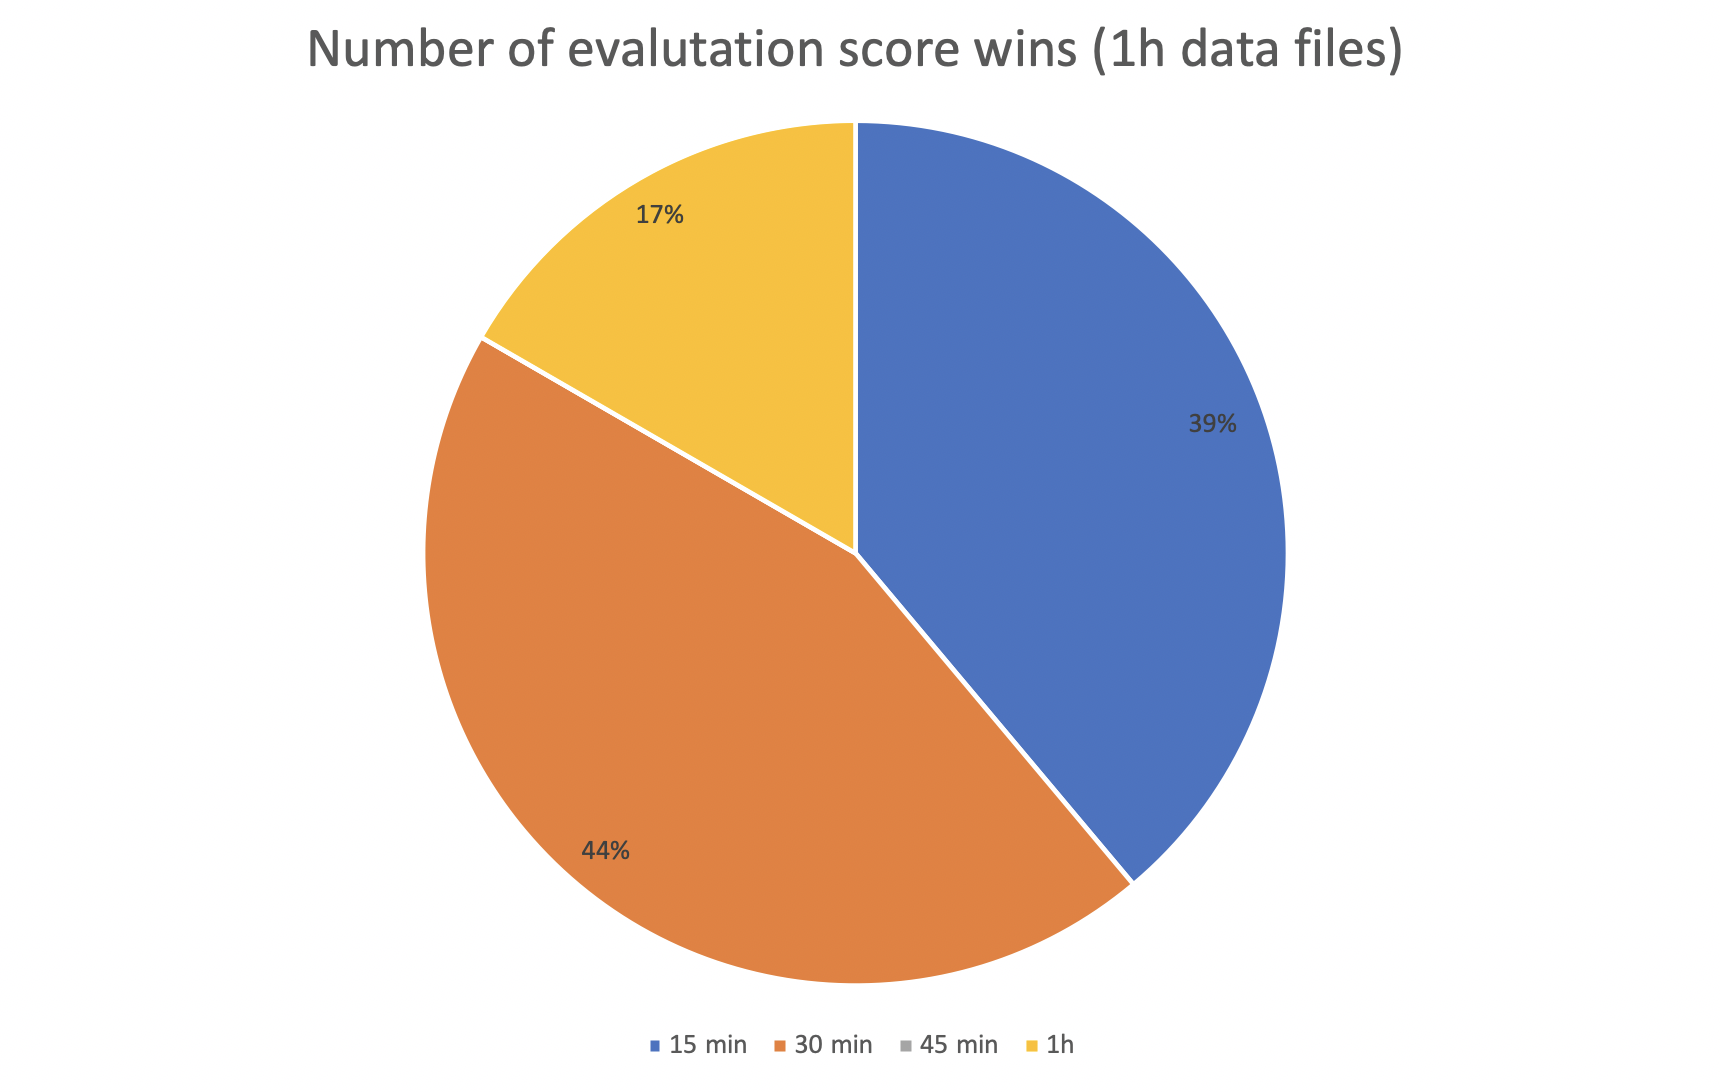
\includegraphics[width=0.8\textwidth]{./images/clusteringResults/clusteringResultsGraph1h.png}
%   \caption{Number of light green evaluation score "wins" (1h or 3h) for the 1h data files.}
%   \label{figure:clusteringResultsGraph1h}
% \end{figure}

% \begin{figure}
%   \centering
%   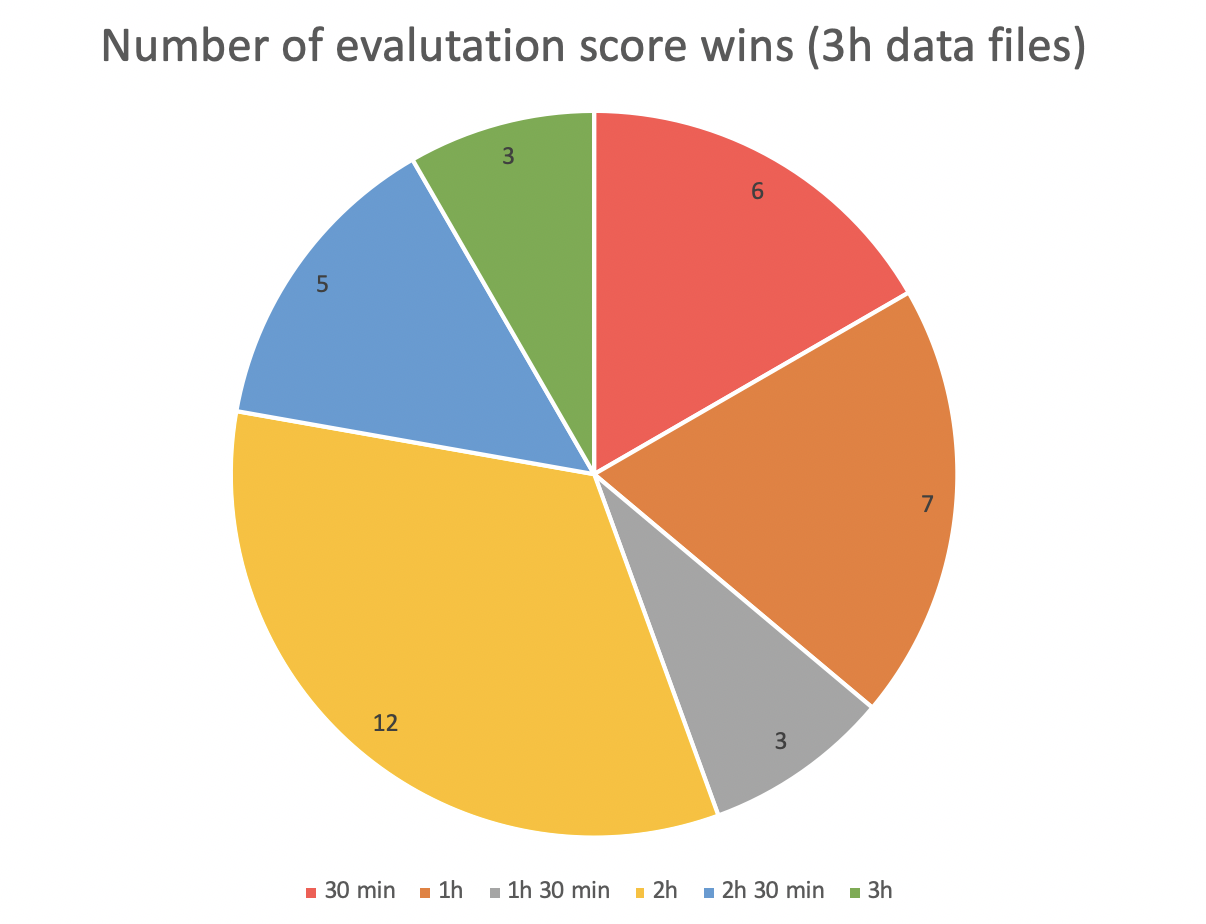
\includegraphics[width=0.8\textwidth]{./images/clusteringResults/clusteringResultsGraph3h.png}
%   \caption{Number of light green evaluation score "wins" (1h or 3h) for the 3h data files.}
%   \label{figure:clusteringResultsGraph3h}
% \end{figure}

\begin{figure}
  \centering
  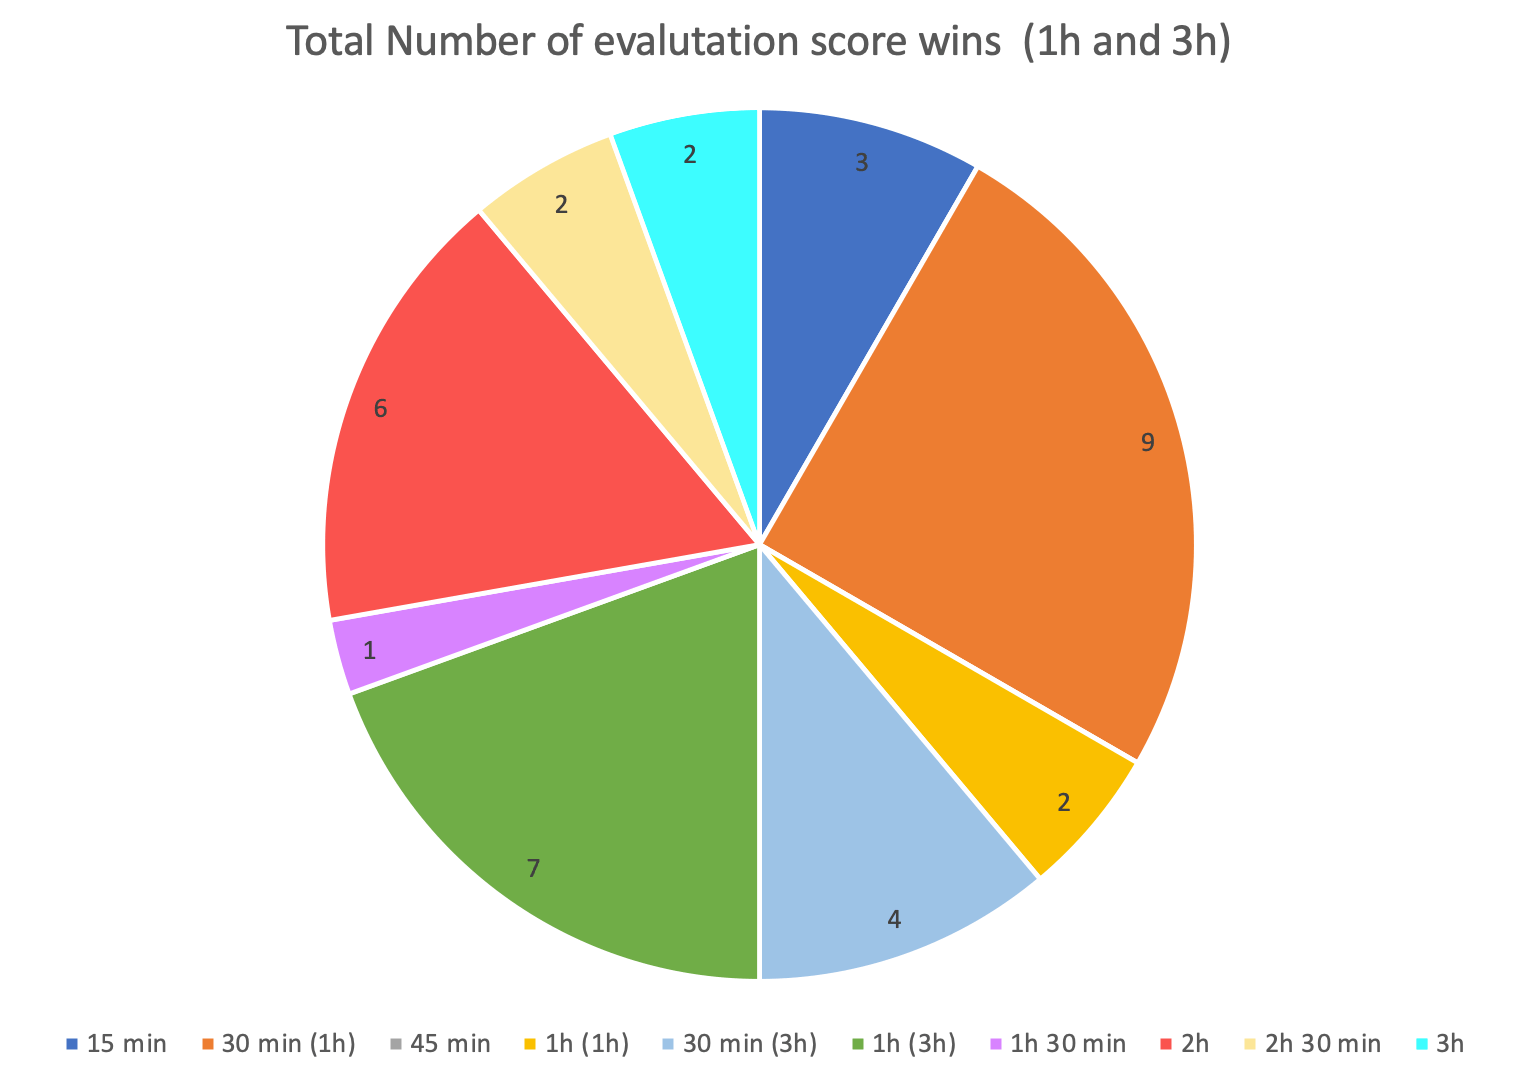
\includegraphics[width=0.5\textwidth]{./images/clusteringResults/clusteringResultsGraphTotal.png}
  \caption{Number of dark green evaluation score "wins" (1h and 3h).}
  \label{figure:clusteringResultsGraphTotal}
\end{figure}






% \begin{figure}
%   \centering
%   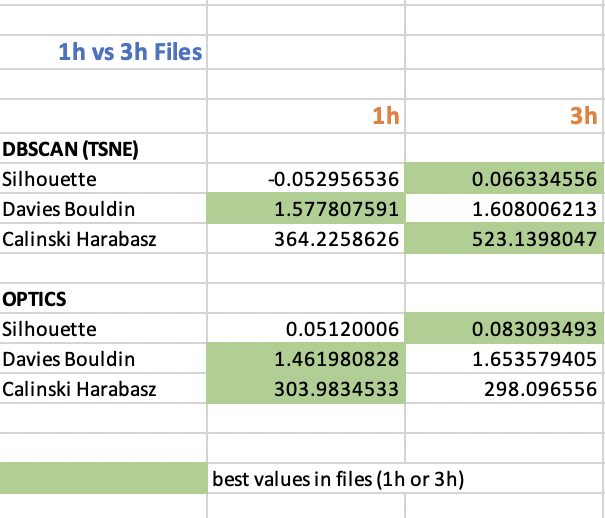
\includegraphics[width=0.8\textwidth]{./images/clusteringResults/clusteringResults7.png}
%   \caption{Evaluation scores comparison from averaged 1h and 3h run of t-SNE and clustering.}
%   \label{figure:clusteringResults7}
% \end{figure}



\begin{figure}
  \centering
  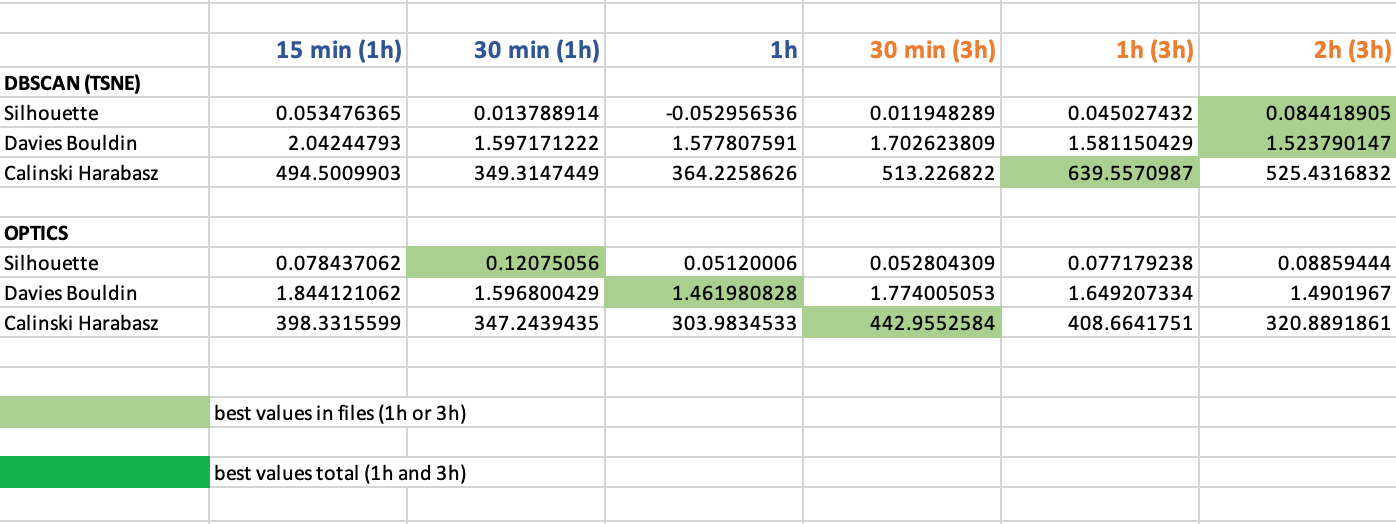
\includegraphics[width=0.8\textwidth]{./images/clusteringResults/clusteringResults8.png}
  \caption{Top evaluation scores performers comparison from figures \ref{figure:clusteringResultsGraph1h}, \ref{figure:clusteringResultsGraph3h}, and \ref{figure:clusteringResultsGraphTotal}.}
  \label{figure:clusteringResults8}
\end{figure}

% \begin{figure}
%   \centering
%   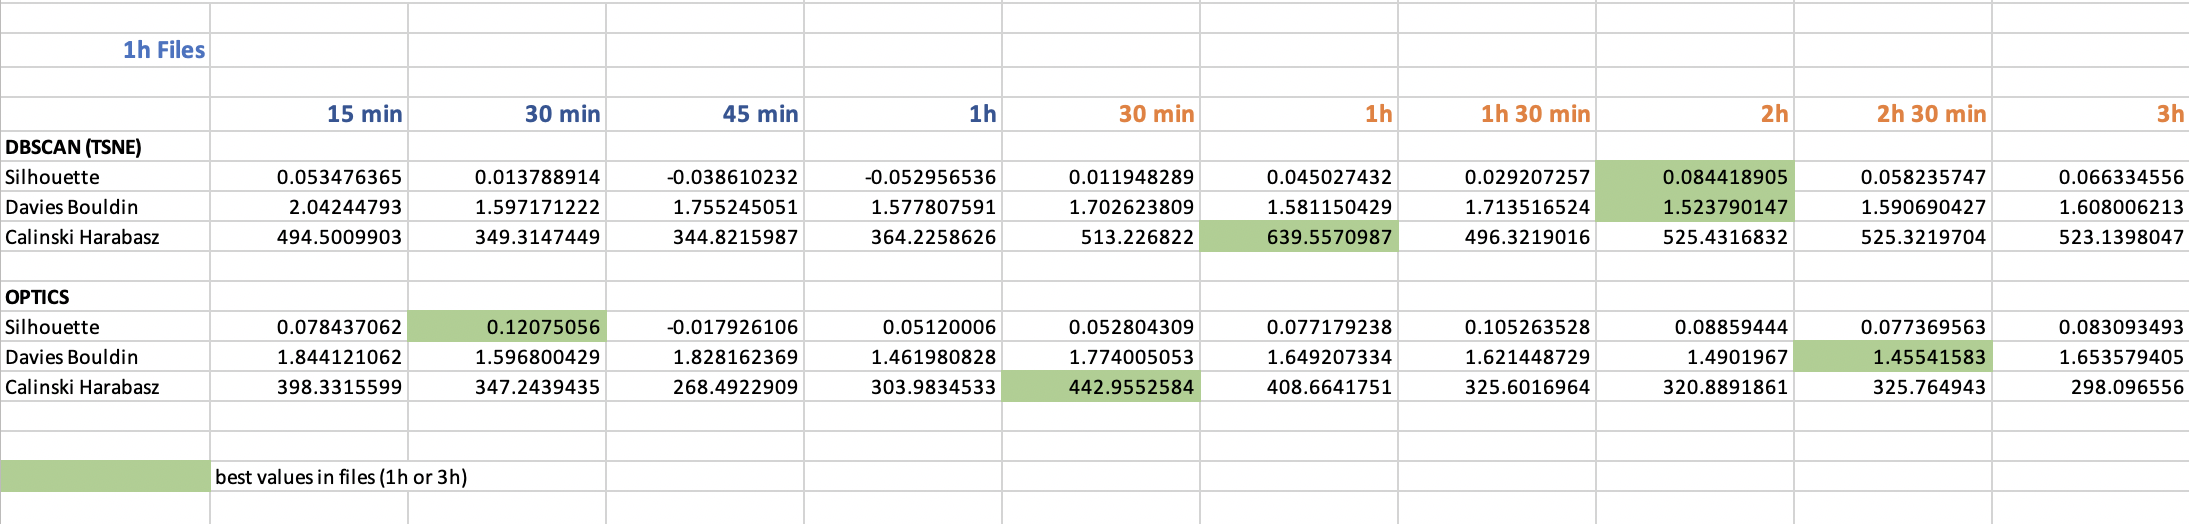
\includegraphics[width=0.8\textwidth]{./images/clusteringResults/clusteringResults9.png}
%   \caption{\textbf{TODO: DON'T THINK NEED THIS.}}
%   \label{figure:clusteringResults9}
% \end{figure}
